% =====================================================================
%  TEC-Vorlage -- Thomas Michael Resch (A01832776)
%  Für jeden neuen Bericht nur den Block "DOKUMENTDATEN" ändern.
%  Das Logo tec_logo.png muss im selben Ordner wie diese Datei liegen.
% =====================================================================
\documentclass[11pt,a4paper]{article}

% ---------- Pakete ----------
\usepackage[utf8]{inputenc}
\usepackage[T1]{fontenc}
\usepackage{lmodern}
\usepackage[english]{babel}
\usepackage{graphicx}
\usepackage{amsmath,amssymb}
\usepackage{booktabs}
\usepackage{float}
\usepackage{etoolbox}
\usepackage[hidelinks]{hyperref}

% ---------- Zusätzliche Pakete (für diesen Bericht) ----------
\usepackage[a4paper,margin=2.54cm]{geometry}   % Normal margins (2.54 cm)
\usepackage{xcolor}
\usepackage{listings}
\lstset{language=Matlab, basicstyle=\ttfamily\scriptsize, breaklines=true, columns=fullflexible,
  frame=single, rulecolor=\color{black!25}, backgroundcolor=\color{black!3}, showstringspaces=false,
  keywordstyle=\color{blue!70!black}, commentstyle=\color{green!45!black}, stringstyle=\color{red!60!black}}

% ---------- Feste Einstellungen ----------
% Jede Section beginnt immer auf einer neuen Seite (auch \section*):
\let\TEColdsection\section
\renewcommand{\section}{\clearpage\TEColdsection}

% ---------- DOKUMENTDATEN (nur diesen Block ändern) ----------
\newcommand{\doctitle}{Activity 2.6}
\newcommand{\docsubtitle}{Position and Speed Control Loop}   % leer lassen = Zeile entfällt
\newcommand{\course}{Industrial Automation -- MR2006B.602}
\newcommand{\coursemodule}{Module 2: Microcontrollers}                        % leer lassen = Zeile entfällt
\newcommand{\professor}{Prof. Federico Guedea}
% -------------------------------------------------------------

\begin{document}

%--------------------------------------------------
% Cover page
\begin{titlepage}
  \centering
  \vspace*{1cm}
  
\includegraphics[width=0.5\textwidth]{tec_logo.png}\par
  \vspace{2cm}
  {\LARGE\bfseries \doctitle\par}
  \ifdefempty{\docsubtitle}{}{\vspace{0.3cm}{\large \docsubtitle\par}}
  \vspace{1.5cm}
  Block name: \course\par
  \ifdefempty{\coursemodule}{}{\vspace{0.2cm}\coursemodule\par}
  \vspace{0.2cm}
  \professor\par
  \vspace{2cm}
  Students:\par
  \vspace{0.2cm}
  Isaac Sebastian Hovmand - A01832781\par
  Thomas Micheal Resch - A01832776\par
  Jan Mosler - A01833812\par
  Daniel Appel - A01833285\par
  \vfill
  Date: \today\par
\end{titlepage}

%--------------------------------------------------
% INHALT
%--------------------------------------------------

\section{Introduction}
This report covers the position and speed control of the car.
First, the plant is identified from open-loop tests.
Then a PID controller is designed, tuned and discretized in MATLAB/Simulink.
Finally, it runs on the NUCLEO-F446RE.
The car drives a target distance with a trapezoidal speed profile.
It stops at obstacles closer than \(30\,\mathrm{mm}\) and receives new parameters via Bluetooth.

% ---------------------------------------------------------------------
\section{Open-Loop Tests}
The motors were driven with fixed PWM duty steps, without feedback.
The encoders were sampled every \(20\,\mathrm{ms}\).
Speed and distance were logged for each step.

\begin{table}[H]
  \centering
  \caption{Open-loop step tests.}
  \begin{tabular}{@{}ccc@{}}
    \toprule
    \textbf{Duty [\%]} & \textbf{Final speed [mm/s]} & \textbf{Time to 63\,\% [s]} \\ \midrule
    20  & [TBD] & [TBD] \\
    40  & [TBD] & [TBD] \\
    60  & [TBD] & [TBD] \\
    80  & [TBD] & [TBD] \\
    100 & 650   & [TBD] \\ \bottomrule
  \end{tabular}
\end{table}

The car starts moving at \(14.1\,\%\) duty (left) and \(16.9\,\%\) duty (right).
Below these values, static friction holds the wheels.

\begin{figure}[H]
  \centering
  \fbox{\parbox[c][4cm][c]{0.8\linewidth}{\centering Open-loop step response (speed vs.\ time)}}
  % \includegraphics[width=0.8\linewidth]{openloop.png}
  \caption{Open-loop step response.}
\end{figure}

% ---------------------------------------------------------------------
\section{Model Identification}
Input \(u\) is the PWM duty in \%. Output \(v\) is the wheel speed in mm/s.
The MATLAB System Identification app estimated a first-order model:
\begin{equation}
  G(s) = \frac{V(s)}{U(s)} = \frac{K}{\tau s + 1}
\end{equation}
with \(K = 7.596\,\mathrm{mm/(s\cdot\%)}\), \(\tau = 0.050\) s and a fit of [TBD] \%.
The dead zone is \(u_0 = 7.0\,\%\).
The position is the integral of the speed:
\begin{equation}
  X(s) = \frac{G(s)}{s}\,U(s)
\end{equation}

\begin{figure}[H]
  \centering
  \fbox{\parbox[c][4cm][c]{0.8\linewidth}{\centering Screenshot: System Identification app}}
  % \includegraphics[width=0.8\linewidth]{sysid.png}
  \caption{Model estimation in the System Identification app.}
\end{figure}

% ---------------------------------------------------------------------
\section{Control Loop Simulation}

\subsection{Closed Loop in Simulink}
The loop has five blocks: reference generator, PID, actuator, plant and sensor.
\begin{itemize}
  \item \textbf{Actuator:} H-bridge. Duty limited to \(\pm 100\,\%\).
  \item \textbf{Plant:} \(G(s)\) from the identification.
  \item \textbf{Sensor:} encoder with gain \(k_x\), sampled every \(T_s\).
\end{itemize}

The reference is a trapezoidal speed profile.
The user sets the distance \(D\), the maximum speed \(v_{max}\),
the acceleration time \(t_a\) and the deceleration time \(t_d\):
\begin{equation}
  v_{ref}(t) =
  \begin{cases}
    v_{max}\,\dfrac{t}{t_a}       & 0 \le t < t_a \\[4pt]
    v_{max}                        & t_a \le t < T - t_d \\[4pt]
    v_{max}\,\dfrac{T - t}{t_d}   & T - t_d \le t \le T
  \end{cases}
\end{equation}
\begin{equation}
  T = \frac{D}{v_{max}} + \frac{t_a + t_d}{2},
  \qquad
  x_{ref}(t) = \int_0^t v_{ref}(\tau)\,d\tau
\end{equation}

\begin{figure}[H]
  \centering
  \fbox{\parbox[c][4cm][c]{0.8\linewidth}{\centering Screenshot: Simulink model}}
  % \includegraphics[width=0.9\linewidth]{simulink.png}
  \caption{Closed control loop in Simulink.}
\end{figure}

\subsection{Continuous PID}
\begin{equation}
  C(s) = K_p + \frac{K_i}{s} + K_d\,s
\end{equation}

\subsection{Discretization}
The sampling time is \(T_s = 20\,\mathrm{ms}\).
It is much smaller than \(\tau\) (rule of thumb: \(T_s \le \tau/10\)).
It also matches the TIM6 interrupt on the microcontroller.
The plant was discretized with a zero-order hold.
The discrete PI uses the forward Euler integral, as in the firmware:
\begin{equation}
  C(z) = K_p + \frac{K_i\,T_s}{z-1}
\end{equation}

\subsection{Tuning}
The PI gains follow the SIMC rules (Skogestad).
Sampling (\(T_s\)) and the speed filter (\(\tau_f = 28.9\,\mathrm{ms}\)) act as a delay
\(\theta = T_s + \tau_f = 49\,\mathrm{ms}\):
\begin{equation}
  K_p = \frac{\tau}{K(\tau_c + \theta)}, \qquad
  T_i = \min\bigl(\tau,\ 4(\tau_c + \theta)\bigr), \qquad
  K_i = \frac{K_p}{T_i}
\end{equation}
The setting \(\tau_c = 2\theta\) (balanced) was chosen: no overshoot, settling in 0.31 s.
\(K_d = 0\). A derivative term would amplify the speed quantization of 3.18 mm/s.
The MATLAB script is in Appendix~\ref{app:code}, its output in Appendix~\ref{app:output}.

\begin{table}[H]
  \centering
  \caption{PI gains (\(K_p\) in \%/(mm/s), \(K_i\) in \%/(mm/s\(\cdot\)s)).}
  \begin{tabular}{@{}lccc@{}}
    \toprule
               & \(K_p\) & \(K_i\) & \(K_d\) \\ \midrule
    Continuous & 0.045   & 0.898   & 0       \\
    Discrete   & 0.045   & 0.898 (\(K_i T_s = 0.018\)) & 0 \\ \bottomrule
  \end{tabular}
\end{table}

\subsection{Validation}
The continuous and the discrete loop give nearly the same response.
In the 1000 mm move (300 mm/s, ramps of 1 s), the discrete loop is within 2 mm
after 4.88 s. The profile takes 4.33 s.
With \(\pm 20\,\%\) plant gain, the final error stays below 1.5 mm.

\begin{table}[H]
  \centering
  \caption{Simulation results.}
  \begin{tabular}{@{}lcc@{}}
    \toprule
    & \textbf{Continuous} & \textbf{Discrete} \\ \midrule
    Overshoot [\%]          & 0.0   & 0.3   \\
    Settling time (5\,\%) [s] & 0.31 & 0.28 \\
    Final position error, 1000 mm move [mm] & \(-0.38\) & 0.88 \\ \bottomrule
  \end{tabular}
\end{table}

\begin{figure}[H]
  \centering
  \fbox{\parbox[c][4cm][c]{0.8\linewidth}{\centering Plot: continuous vs.\ discrete response}}
  % 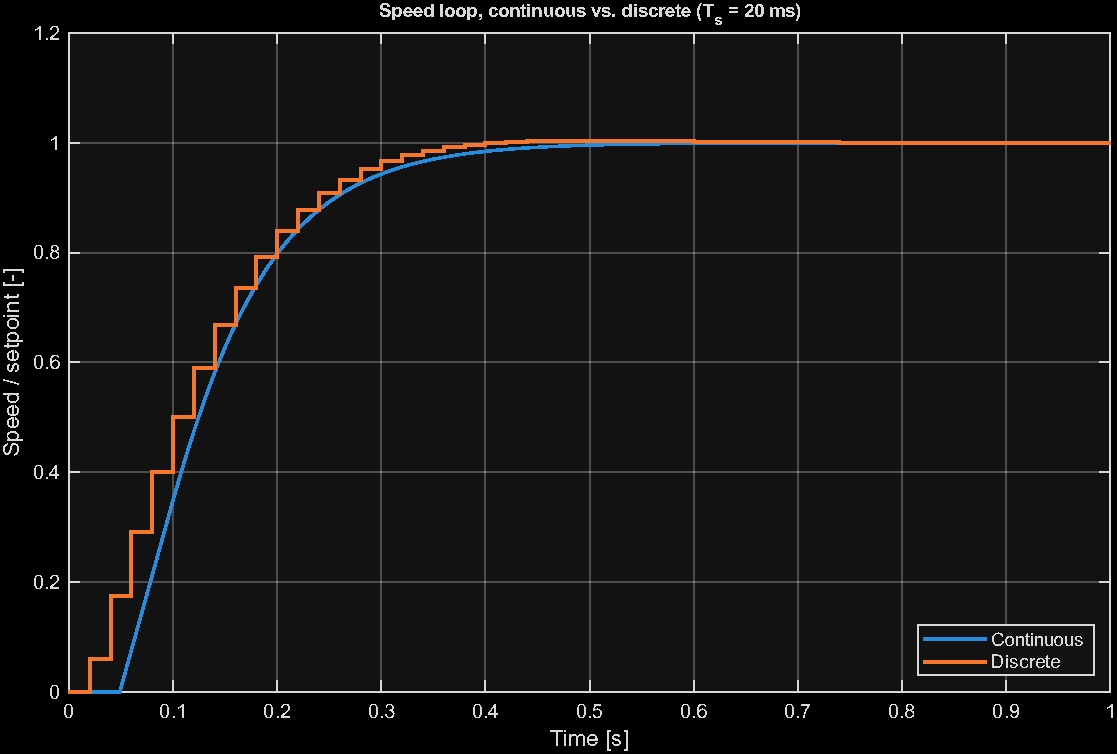
\includegraphics[width=0.8\linewidth]{fig_cont_vs_disc.pdf}
  \caption{Continuous and discrete simulation.}
\end{figure}

% ---------------------------------------------------------------------
\section{Hardware}
% TODO: confirm module models and fill in the new pins.
\begin{table}[H]
  \centering
  \caption{Sensors, actuators and interfaces.}
  \small
  \begin{tabular}{@{}lll@{}}
    \toprule
    \textbf{Device} & \textbf{Interface} & \textbf{Pins} \\ \midrule
    2\(\times\) BTS7960 H-bridge   & PWM (TIM1)          & PA8--PA11, PB12/13 (EN) \\
    2\(\times\) motor encoder      & Encoder (TIM3/TIM8) & PA6, PA7; PC6, PC7 \\
    Ultrasonic sensor             & GPIO (trig/echo)    & [TBD] \\
    OLED display                  & I\textsuperscript{2}C & [TBD] \\
    Bluetooth module              & UART                & [TBD] \\ \bottomrule
  \end{tabular}
\end{table}

\begin{figure}[H]
  \centering
  \fbox{\parbox[c][5cm][c]{0.8\linewidth}{\centering Schematic of the car}}
  % \includegraphics[width=0.9\linewidth]{schematic.png}
  \caption{Wiring of the car.}
\end{figure}

% ---------------------------------------------------------------------
\section{Firmware Implementation}

\subsection{Sampling Period}
TIM6 runs at \(f_{TIM6} = 90\,\mathrm{MHz}\) (APB1 \(45\,\mathrm{MHz} \times 2\)).
With PSC \(= 8999\) and ARR \(= 199\):
\begin{equation}
  f_s = \frac{f_{TIM6}}{(PSC+1)(ARR+1)} = \frac{90\cdot 10^6\,\mathrm{Hz}}{9000 \cdot 200} = 50\,\mathrm{Hz}
\end{equation}
\begin{equation}
  T_s = \frac{1}{f_s} = 20\,\mathrm{ms}
\end{equation}

\subsection{PWM Signal}
% TODO: check APB2 timer clock and PSC/ARR of TIM1 in the .ioc file.
TIM1 generates the PWM for both H-bridges at \(20\,\mathrm{kHz}\).
\begin{equation}
  f_{PWM} = \frac{f_{TIM1}}{(PSC+1)(ARR+1)}
\end{equation}
\begin{equation}
  (PSC+1)(ARR+1) = \frac{180\cdot 10^6\,\mathrm{Hz}}{20\cdot 10^3\,\mathrm{Hz}} = 9000
\end{equation}
\begin{equation}
  \text{Duty} = \frac{CCR}{ARR+1} \cdot 100\,\%
\end{equation}
Used values: PSC \(=\) [TBD], ARR \(=\) [TBD].

\subsection{Distance and Speed}
Each encoder gives \(N_{rev} = 3584\) counts per wheel revolution (x4 decoding).
The wheel circumference is \(C_w \approx 228\,\mathrm{mm}\).
\begin{equation}
  k_x = \frac{C_w}{N_{rev}} = \frac{228}{3584} \approx 0.0636\,\mathrm{mm/count}
\end{equation}
\begin{equation}
  x[k] = k_x\,N[k],
  \qquad
  v[k] = \frac{x[k] - x[k-1]}{T_s}
\end{equation}
The speed resolution is \(k_x / T_s \approx 3.18\,\mathrm{mm/s}\).

\subsection{PID Algorithm}
The PID runs in the TIM6 callback, every \(T_s\):
\begin{align}
  e[k] &= r[k] - y[k] \\
  I[k] &= I[k-1] + K_i\,T_s\,e[k] \\
  u[k] &= K_p\,e[k] + I[k] + K_d\,\frac{e[k] - e[k-1]}{T_s}
\end{align}
The output is limited to \(\pm 100\,\%\) duty.
When the output saturates, the integral stops (anti-windup).

\begin{verbatim}
TIM6 callback (every 20 ms):
  read encoders            -> x, v
  next reference point     -> x_ref, v_ref
  if obstacle: hold reference, duty = 0
  else:        PID -> duty -> CCR (TIM1)
\end{verbatim}

\subsection{OLED Display}
% TODO: confirm what is shown and where it is refreshed.
The OLED shows the state (run / stop / obstacle), the target distance,
the current distance and speed, and the PID gains.
It is refreshed in the main loop, outside the interrupt.

\subsection{Bluetooth}
% TODO: match commands and baud rate to the code.
Parameters are sent from a phone via the Bluetooth module (UART, [TBD] baud).

\begin{table}[H]
  \centering
  \caption{Bluetooth commands.}
  \begin{tabular}{@{}ll@{}}
    \toprule
    \textbf{Command} & \textbf{Function} \\ \midrule
    \texttt{D<mm>}   & Set target distance and start \\
    {[TBD]}          & Set \(K_p\), \(K_i\), \(K_d\) \\
    {[TBD]}          & Set \(v_{max}\), \(t_a\), \(t_d\) \\ \bottomrule
  \end{tabular}
\end{table}

\subsection{Obstacle Detection}
The ultrasonic sensor measures the echo time \(t_{echo}\).
With the speed of sound \(c = 343\,\mathrm{m/s}\):
\begin{equation}
  d = \frac{c\,t_{echo}}{2}
  \;\Rightarrow\;
  d\,[\mathrm{mm}] = 0.1715 \cdot t_{echo}\,[\mu\mathrm{s}]
\end{equation}
If \(d \le 30\,\mathrm{mm}\), the motors stop and the reference is held.
When the obstacle is removed, the car continues the profile.

% ---------------------------------------------------------------------
\section{Results}

\subsection{STM32CubeMonitor vs.\ MATLAB}
\begin{figure}[H]
  \centering
  \fbox{\parbox[c][4cm][c]{0.8\linewidth}{\centering Screenshot: STM32CubeMonitor vs.\ simulation}}
  % \includegraphics[width=0.8\linewidth]{cubemonitor.png}
  \caption{Measured and simulated response.}
\end{figure}

\begin{table}[H]
  \centering
  \caption{Simulation and measurement.}
  \begin{tabular}{@{}lcc@{}}
    \toprule
    & \textbf{Simulation} & \textbf{Measured} \\ \midrule
    Target distance [mm]   & [TBD] & [TBD] \\
    Distance traveled [mm] & [TBD] & [TBD] \\
    Maximum speed [mm/s]   & [TBD] & [TBD] \\
    Travel time [s]        & [TBD] & [TBD] \\ \bottomrule
  \end{tabular}
\end{table}

\subsection{Obstacle Test}
An obstacle was placed in front of the car during a move.
The car stopped at [TBD] mm and continued after the obstacle was removed.

% ---------------------------------------------------------------------
\section{Conclusions}
% TODO: write after the tests.
[TBD]

% ---------------------------------------------------------------------
\appendix
\section{MATLAB Code}\label{app:code}
\lstinputlisting{identify_car.m}

\section{MATLAB Output}\label{app:output}
\lstinputlisting[language={}, columns=fixed, basewidth=0.5em, basicstyle=\ttfamily\fontsize{6.5}{8}\selectfont]{identify_car_output.txt}

\end{document}
